\documentclass[useAMS,usenatbib]{mn2e}
\usepackage{graphicx}
\usepackage{url}
%\usepackage{tikz}
\newcommand{\aap}{Astron. Astrophys.}
\newcommand{\aj}{Astron. J.}
\newcommand{\ao}{Appl. Opt.}
\newcommand{\apj}{Astrophys. J.}
\newcommand{\apjl}{Astrophys. J. Lett.}
\newcommand{\apjs}{Astrophys. J. Suppl.}
\newcommand{\mnras}{Mon. Not. Roy. Ast. Soc.}
\newcommand{\nat}{Nature}
\newcommand{\pasa}{Publ. Ast. Soc. Aust.}
\newcommand{\pasp}{Publ. Ast. Soc. Pac.}
\newcommand{\prl}{Phys. Rev. Lett.}
\newcommand{\prd}{Phys. Rev. D}
\newcommand{\msun}{\mathrm{M}_\odot}

\title[2MPZ and LIGO]{Using the 2-MASS Photometric Redshift Survey to optimize LIGO Follow-Up Observations}
\author[Antolini \& Heyl]{Elisa Antolini$^{1}$, Jeremy S. Heyl$\thanks{Email:
    heyl@phas.ubc.ca; Canada Research Chair}$^{2}$ \\
  $^{1}$Dipartimento di Fisica e Geologia, Universit\`a degli Studi di Perugia, I-06123 Perugia, Italia \\
  $^{2}$Department of Physics and Astronomy, University of British
  Columbia, 6224 Agricultural Road, Vancouver, BC V6T 1Z1, Canada\\
}
\begin{document}
\date{Accepted ---. Received ---; in original form ---}

\pagerange{\pageref{firstpage}--\pageref{lastpage}} \pubyear{2015}

\maketitle

\label{firstpage}

\begin{abstract}
  The initial discovery of LIGO on 14 September 2015 was the in-spiral
  merger and ring-down of the black hole binary at a distance of about
  500~Mpc or a redshift of about 0.1.  The search for electromagnetic
  counterparts for such sources is impeded by poor initial source
  localizations and a lack of a compelling model for the counterpart
  Because astrophysical sources of gravitational radiation are likely
  to reside in galaxies, it would make sense to search first in
  regions where the LIGO-Virgo probability is large and where the
  density of galaxies is large as well.  Under the Bayesian prior
  assumption that the probability of a gravitational-wave event from a
  given region of space is proportional to the density of galaxies
  within the probed volume, one can calculate an improved localization
  of the position of the source simply by multiplying the LIGO-Virgo
  skymap by the density of galaxies in the range of redshifts.  We
  propose using the 2-MASS Photometric Redshift Galaxy Catalogue for
  this purpose and demonstrate that using it can dramtically reduce
  the search region for electromagnetic counterparts.
\end{abstract}

\section{Introduction}

LIGO has recently begun to detect gravitational wave events from the
local Universe \citep{PhysRevLett.116.061102}.  During these initial
years of gravitational astronomy, the localization of the candidate
events on the sky is poor with the ninety-percent confidence regions
covering hundreds or even thousands of square degrees.  Finding an
electromagnetic counterpart to these candidate graviational-wave
events will be crucial to understanding what produces them,
interpretation of the signal and to provide tests of general
relativity.  The ideas of how the the electromagnetic counterparts
would appear are varied and uncertain. There has been substantial
speculation on the electromagnetic transients associated with the
mergers of binaries that include a neutron star
\citep[e.g.][]{2016PhRvD..93b4011E,2016arXiv160107711K,2016arXiv160100017D,2015arXiv151205435F,2015ApJ...814L..20M,2015PhRvD..92d4028K,2015arXiv150807939S,2015arXiv150807911S}
However,the first discovered gravitational wave event appears to be
the merger of binary black holes, so the appearance and duration of
the electromagnetic counterparts are especially uncertain with only a few models
\citep[e.g.][]{2015PhRvL.115n1102G,2015MNRAS.452.3419M,2016MNRAS.457..939C,2016ApJ...817..183Y}
Consequently, rapid electromagnetic follow-up of a large portion of
the probable region would increase the chance of success in finding a
counterpart.  Over the large search regions and over the span of days
or weeks, many electromagnetic transients typically occur, and with
the wide variety of models it will be difficult to associate
unambigously a particular electromagnetic event with a candidate
gravitational-wave event.

The purpose of this letter is to present a strategy to alleviate both
of these issues; that is, to reduce both the search region and the
time required to plan and begin observations.  We follow the spirit of
\citet{2015arXiv150803608G} to develop a galaxy catalogue to guide the
observational plan.  However, our goal here is to develop a nearly
complete catalogue at the expense of having less accurate estimates of
the redshifts of the galaxies within the catalogue.  The accuracy of
the galaxy distances needs to be only as good as the distance estmates
of the gravitational-wave events.  Additionally we will outline a
straightforward and rapid technique to generate a nearly optimal
observing plan to follow up the events rapidly (i.e. within a few
seconds of the trigger). 

\section{Bayesian Approach to Follow-Up}

Because we will be interested in the rapid follow-up of candidate
gravitational-wave events, we will focussed on the rapid Bayesian
reconsruction outlined by \citet{2015arXiv150803634S}, BAYESTAR.  At
the most basic level, BAYESTAR yields a probability map on the sky in
the form of a HEALPpix map \citep{2005ApJ...622..759G} where each
pixel contains the probability $P(d|m)$ that a particular model
(i.e. position on the sky) will yield the data (i.e. the observed
strains on the LIGO and Virgo interferometers).  To plan an observing
strategy one would like the probability of a particular model
(i.e. position on the sky) given the data.  We have from Bayes's
theorem
\begin{equation}
  P(\mathrm{position}|\mathrm{data}) = \frac{P(\mathrm{position})
    P(\mathrm{data}|\mathrm{position})}{P(\mathrm{data})}.
  \label{eq:1}
\end{equation}
If we make the additional mild assumption that gravitational-waves
originate from nearby galaxies, the probability of a given position on
the sky naturally is proportional to the density (or perhaps the
luminosity density) of galaxies in that direction integrated over
distance range determined from the modelling of the gravitational
waveform.  Of course, these distance estimates will usually have large
uncertainities so the distance range over which to integrate the
galaxy density distribution will also be large, so highly accurate
redshift information is not needed to construct
$P(\mathrm{position})$.

Furthermore, because we will ultimately be interested in which fields
to observe (not which particular galaxies), accurate positions are not
required in the construction of $P(\mathrm{position})$. It is natural
to sample $P(\mathrm{position})$ also as a HEALPix grid with each pixel
covering about the same solid angle as the field of view of the
telescope of interest or the BAYESTAR map (a HEALPix level of 512 or
about 50 square arcminutes per pixel), so positions no more accurate
than arcminutes are required.  The key to generate the observing plan
rapidly is to calculate the required galaxy density maps beforehand in
principle at the desired resolution (this optimization only speeds the
process up slightly) for the distance ranges of interest.  With the
arrival of an alert, all that is required is to calculate
Eq.~(\ref{eq:1}) using the HEALPix maps, resample to the scale of the
telescope, renormalize the probability, sort the pixels from most
likely to least and output the positions to cover a given amount of
cumulative probability (this entire process takes typically less than
one second).

\section{Galaxy Catalogues}

To gain a picture of the local Universe, our focus will be the
completness of the data rather than the accuracy of the distances and
positions.  \citet{2015arXiv150803608G} combine several redshift
surveys
\citep[e.g.][]{2002MNRAS.336..907N,2003MNRAS.344..307L,2005MNRAS.360...81D,
  2012ApJS..199...26H}
that cover a large portion of the sky, but at various depths and
attempt to increasing the completeness of the sample by using only the
galaxies near the upper-end of the luminosity function ({\em i.e.}
$L\sim L_*$) and ; the discovery that binary black holes with large
masses (!)  dominate the initial detections indicates that focussing
the search on massive galaxies might not be the best strategy.  After
all such large black holes have not been found so far in our
approximately $L_*$-galaxy, the Milky Way, or our neighbour,
Andromeda.  In fact theoretical arguments indicate that the production
of such massive black holes results from the evolution of massive
stars in low metallicity galaxies which are typically small in the
local Universe. Our goal is to have a nearly complete survey that
attempts to be unbiased with respect to the mass of the galaxy.

We follow in spirit the work of \citet{2004PASA...21..396J} who used
The Two Micron All Sky Survey extended source catalogue \citep[2MASS
  XSC,][]{2000AJ....119.2498J,2006AJ....131.1163S}, and the assuption
that all galaxies have the same $K_s-$band luminosity of around $L_*$
to estimate distances to each galaxy and create sky maps of the local
Universe.  A substantial fraction of 2MASS has measured redshifts
\citep[e.g][]{2012ApJS..199...26H}.  \citet{2014ApJS..210....9B}
combined the photometric data from 2MASS XSC with additional
photometry the mid-infrared from WISE \citep{2010AJ....140.1868W} and
the optical from SuperCOSMOS
\citep{2001MNRAS.326.1315H,2001MNRAS.326.1295H,2001MNRAS.326.1279H}.
Using this multiband photometry, they trained neural networks using
measured spectroscopic redshifts from SDSS
\citep{2012ApJS..203...21A,2014ApJS..211...17A}, 2dF
\citep{2001MNRAS.328.1039C,2003astro.ph..6581C}, 6dF
\citep{2004MNRAS.355..747J,2009MNRAS.399..683J} and other catalogues
to determine photometric redshifts.  They also extend the photometric
redshift catalogue beyond the 2MASS XSC building a three-dimensional
map of the sky out to a redshift of nearly 0.2 well into the realm of
the first gravitational wave event.  The 2MASS Photometric Redshift
(2MPZ) catalogue contains over one million galaxies with a median
redshift of 0.1 with a typical scatter between the
photometric and spectroscopic redshifts (where both are known) of
$\sigma_z = 0.015$.

Except for the most local sources, the estimate distances from the
gravitational wave data itself have comparable errors to this, so this
catalogue is sufficiently accurate to calculate the surface density of
galaxies with the expected redshift range of a particular
gravitational-wave detection.  Furthermore, for the nearest sources,
there are nearly uniform all-sky redshift surveys which would be more
appropriate for this task
\citep[e.g]{2000MNRAS.317...55S,2012ApJS..199...26H}.  Of course, all
of the techniques outlined here can be applied to these more nearby
catalogues to produce sky maps of even more nearby galaxies.  Here we
will focus on galaxies with photometric redshifts between 0.01 and 0.1
from the 2MPZ as depicted in Fig.~\ref{fig:galmap}.  For closer
galaxies the redshift error is significant, and the outer end of the
range is both the median redshift of the catalogue and the typical
distances of the binary-black-hole sources.
\begin{figure}
  \includegraphics[width=\columnwidth]{2MPZgz_001_01_smoothed}
  \caption{The relative surface density of galaxies in the 2-MASS Photometric Redshift Survey with photometric redshifts between 0.01 and 0.1, smoothed with a Gaussian of 0.6 degrees (0.01 radian).}
  \label{fig:galmap}
\end{figure}

To produce this map we divided the sky into 3,145,728 regions (each of
about 45 square arcminutes, four ACS fields) using a HEALPix
\citep{2005ApJ...622..759G} tesselation with $\mathtt{NSIDE}=512$.
Each cell of the map simply contains the number of galaxies in the
2MPZ catalogue within the range of photometric redshift that lie
within that portion of sky.  We have subsequently smoothed the map
with a Gaussian with $\sigma=0.01$ radian.  Typically no HEALPix pixel
contains more than one galaxy from the catalogue.  After smoothing we
notice the large-scale structure even when we have averaged over
distance.  This demonstrates the potential optimization in the
observing strategy by observing fields with nearby galaxies. Depending
on whether one believes that the sources are associated with the
visible portion of galaxies or may travel some distance from the
galaxy itself before the gravitational-wave event, one would use
either the raw galaxy counts or the smoothed map.

Furthermore, our choice of weighting the fields simply by the number
of galaxies within each field is perhaps the most simple one.  Given
the type of event, one could use a map that gives small,
low-metallicity galaxies more weight or weigh the galaxies by their
mass or luminosity.  Of course, all of these possibilities would be
informed by one's prior knownledge of the source inspired by
theoretical models and the hints from the waveform itself and give a
better estimate of $P(\mathrm{position})$.  The key is to calculate these
maps beforehand.

There is a further structure apparent in the map, and this is of
course the zone of avoidance imposed by the disk and bulge of our
Galaxy. One can attempt to probe the zone of avoidance
\citep[e.g][]{2000AJ....120..298J} and future 21-cm surveys like CHIME
\citep{2014era..conf10102V} will also probe the large-scale structure
beyond the Galactic plane.  However, the existing galaxy density map
as depicted in Fig.~\ref{fig:galmap} can yield an estimate of the
structure obscured by the Galaxy.
\begin{figure}
  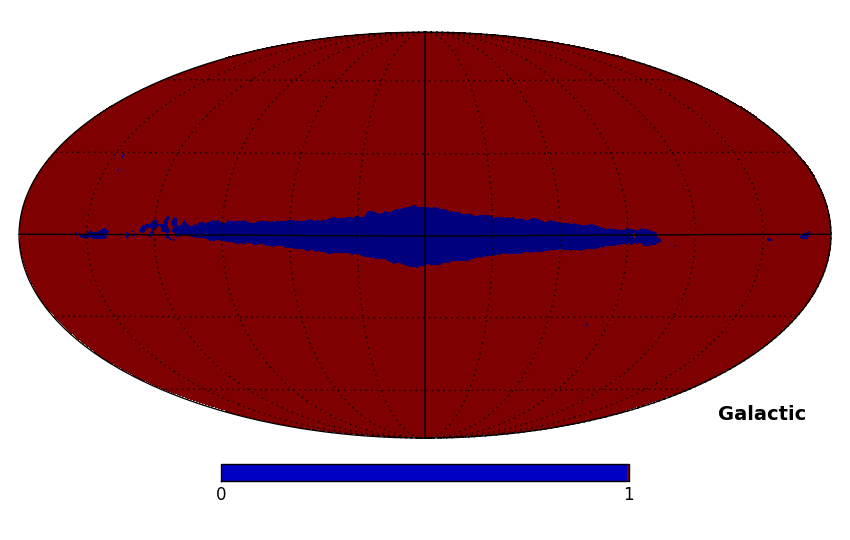
\includegraphics[width=\columnwidth]{test_mask}
  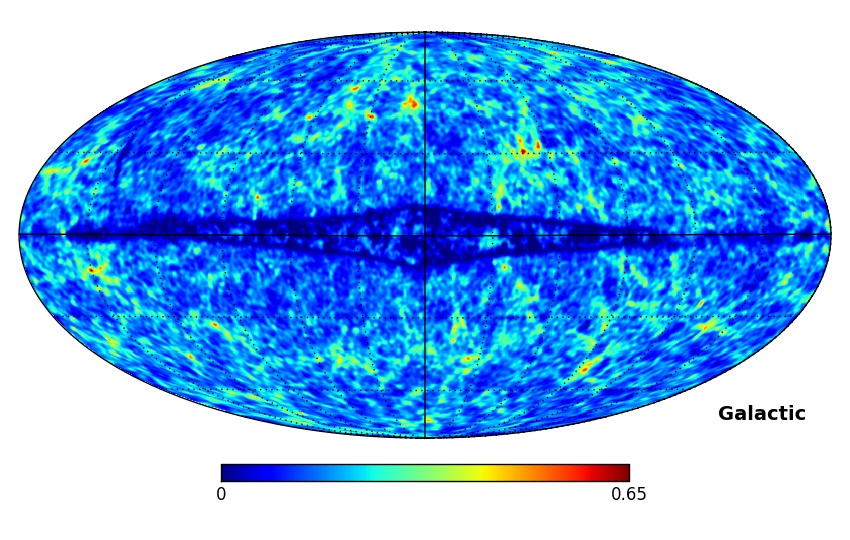
\includegraphics[width=\columnwidth]{combined}
  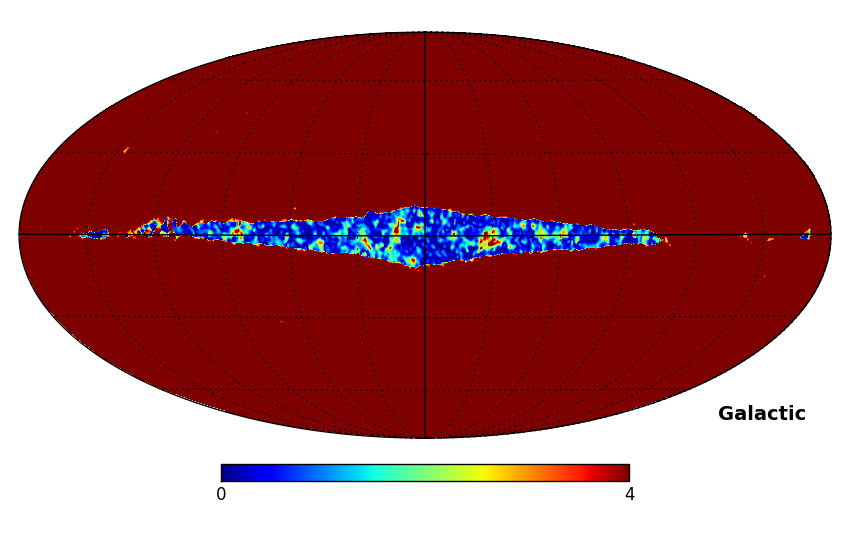
\includegraphics[width=\columnwidth]{snr}
  \caption{Upper: the mask used for the infilling procedure obtained
    by determining the regions where the galaxy density is less than
    one tenth of the mean.  Middle: the infilled galaxy
    distribution. Lower: The signal-to-noise of the infilled map
    obtained by bootstrapping the galaxy catalogue.}
  \label{fig:infilling}
\end{figure}
\section{Results}

\begin{figure}
  \includegraphics[width=\columnwidth,clip,trim=0 1.35cm 0 0]{T125738_bayestar_2MPZgz_003_004.pdf} 
  \includegraphics[width=\columnwidth,clip,trim=0 0 0 0.15cm]{T125738_bayestar_2MPZgz_001_005.pdf} 
  \caption{The number of fields required to cover the given fraction
    of the probablity region for a simulated LIGO detection (red
    curves without the galaxy map, green curves with a smoothed
    galaxy, blue curves with a raw galaxy map).  The upper solid
    curves use a healpix map with about 200,000 cells, the dashed
    curves have about 50,000 cells, the dotted curves have about
    12,000 cells and lower solid curves have about 3,000 cells,
    corresponding 0.2, 0.8, 3.2 and 13 square-degree fields of
    view. The redshift range of the galaxy map in the upper panel is
    $0.03<z<0.04$ and $0.01<z<0.05$ in the lowel panel.}
\end{figure}

\section{Conclusions}

This work was supported by the Natural Sciences and Engineering
Research Council of Canada, the Canadian Foundation for Innovation,
the British Columbia Knowledge Development Fund and the Bertha and
Louis Weinstein Research Fund at the University of British Columbia.


\bibliography{obsplan}
\bibliographystyle{apj}


\label{lastpage}
\end{document}
